	\subsection{Mountain Bike Suspension Concepts}
		The purpose of suspension on a mountain bike is to absorb the energy created from riding over features such as bumps and rough terrain encountered along a trail, improving comfort for the rider and allowing them to go faster by maintaining better contact between the tires and the ground. This requires the use of a spring and damper, collectively known as a shock absorber, which allows the wheel to move away from the feature on contact and make a controlled return once it has been passed.
	\subsubsection{Travel and Stroke}
		\Gls{travel} is the distance which the bike’s fork or frame allow the wheel to move in an upward direction while \gls{stroke} is the distance that the shock absorber can compress before it bottoms out. \Gls{travel} is measured in millimetres or inches and can range from 80mm to 210mm or 4in to 9in. Bikes designed for different disciplines require differing amounts of travel with those designed for cross-country riding typically requiring less travel than those designed for more aggressive disciplines such as downhill racing having more. See Table \ref{tab:travel} for typical specifications.
		\begin{table}[h!]
		\centering
		\caption{Table of common suspension \glspl{travel} and intended disciplines}
		\label{tab:travel}
		\begin{tabular}{|c|cccc|}
			\hline
			Travel (mm)&Cross Country&Trail&Enduro&Downhill\\
			\hline
			80&\cellcolor[gray]{0.5}&&&
			\\
			100&\cellcolor[gray]{0.5}&&&
			\\
			120&\cellcolor[gray]{0.5}&\cellcolor[gray]{0.5}&&
			\\
			140&&\cellcolor[gray]{0.5}&\cellcolor[gray]{0.5}&
			\\
			160&&&\cellcolor[gray]{0.5}&
			\\
			180&&&\cellcolor[gray]{0.5}&\cellcolor[gray]{0.5}
			\\
			+200&&&&\cellcolor[gray]{0.5}\\
			\hline
		\end{tabular}
	\end{table}
	\begin{figure}[h!]
		\centering
		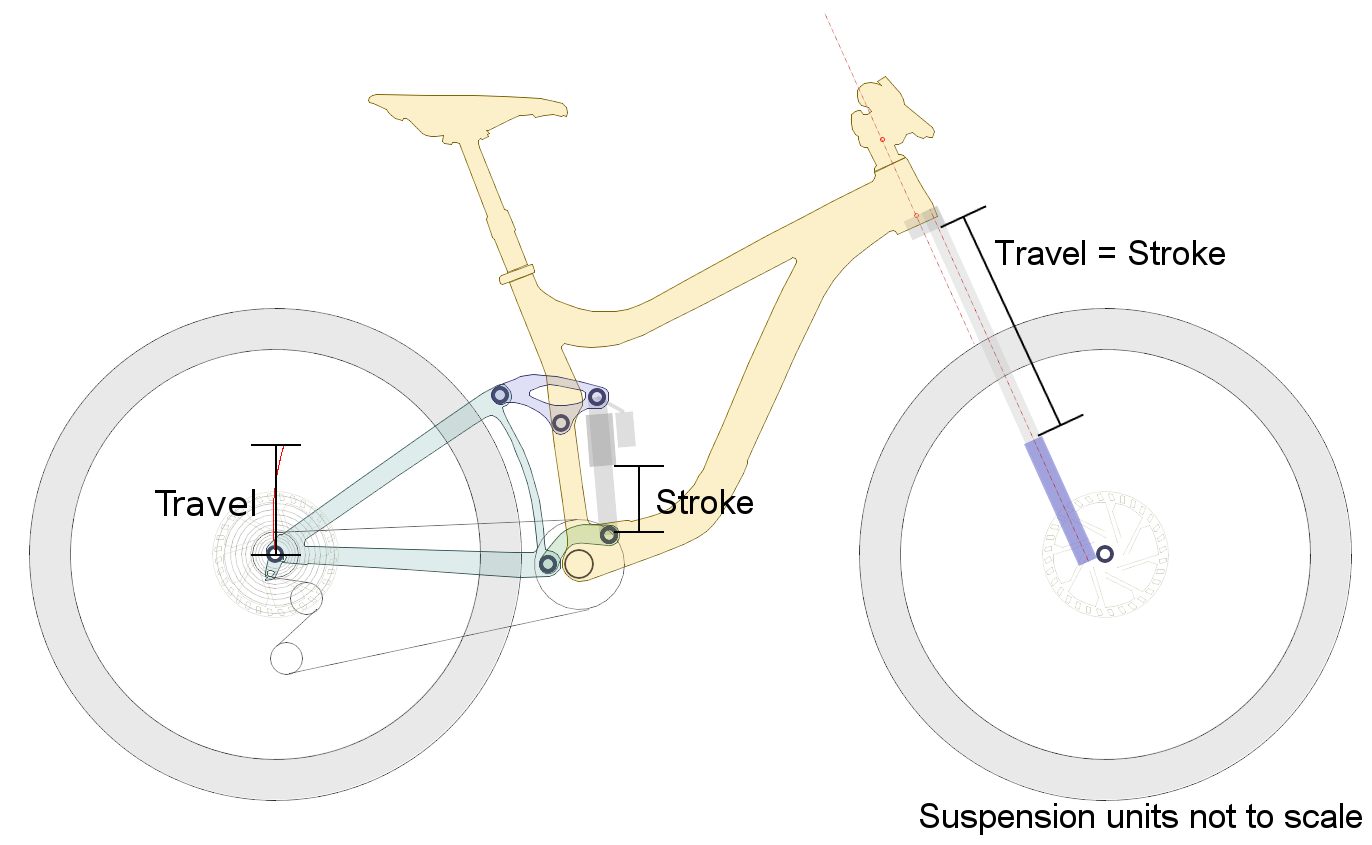
\includegraphics[width=12cm]{../images/reignschpath.PNG}
		\caption[Diagram showing travel and stroke on a full suspension bike]{Diagram showing 
			travel and stroke on a full suspension bike\footnotemark}
		\label{fig:travelvsstroke}
	\end{figure}
	\subsubsection{Front Suspension}
		Front suspension commonly employs a linear telescoping shock absorber, known as a \gls{fork} due to it's dual sided construction. On nearly all suspension \glspl{fork} the \gls{stroke} is 1:1 with the potential travel of the wheel. Front suspension is found on 
		all \gls{fs} and \gls{ht} bikes.
	\subsubsection{Rear Suspension}
		
		Rear suspension uses a shock absorber that is much shorter than a fork so it cannot operate on a 1:1 ratio and still allow the desired travel. Full suspension frames incorporate one or more pivot points and linkages which allow the wheel to move and act as multipliers for the suspension. Rear ratios are expressed as n:1 where n is the average distance the rear wheel moves for every 1mm the shock compresses throughout its stroke; the leverage ratio changing constantly across the compression cycle.
		\\\\
		The difference between front and rear stroke and travel can be seen in Figure \ref{fig:travelvsstroke} noting the separation of rear wheel travel from the stroke of the shock absorber. Although manufacturers design their rear suspension differently, the rear wheel always rotates around the main pivot, (or in some cases a virtual pivot), as opposed to moving linearly as front forks do. As a result, the frame behaves differently through its travel, depending on the number and location of pivot points and the type of shock that it is being used. 
		\\\\
		Because of this the average ratio is normally dismissed in favour of a leverage curve that plots the ratio n:1 throughout the compression cycle. Figure \ref{fig:3_bike_lev_ratio} shows the leverage curves of three modern suspension designs. Each of these designs has between 150mm and 170mm of travel and uses the 27.5 inch wheel size. However, it is evident that varying the location of pivot points produces suspension with drastically different characteristics.
		\begin{figure}[h!]
			\centering
			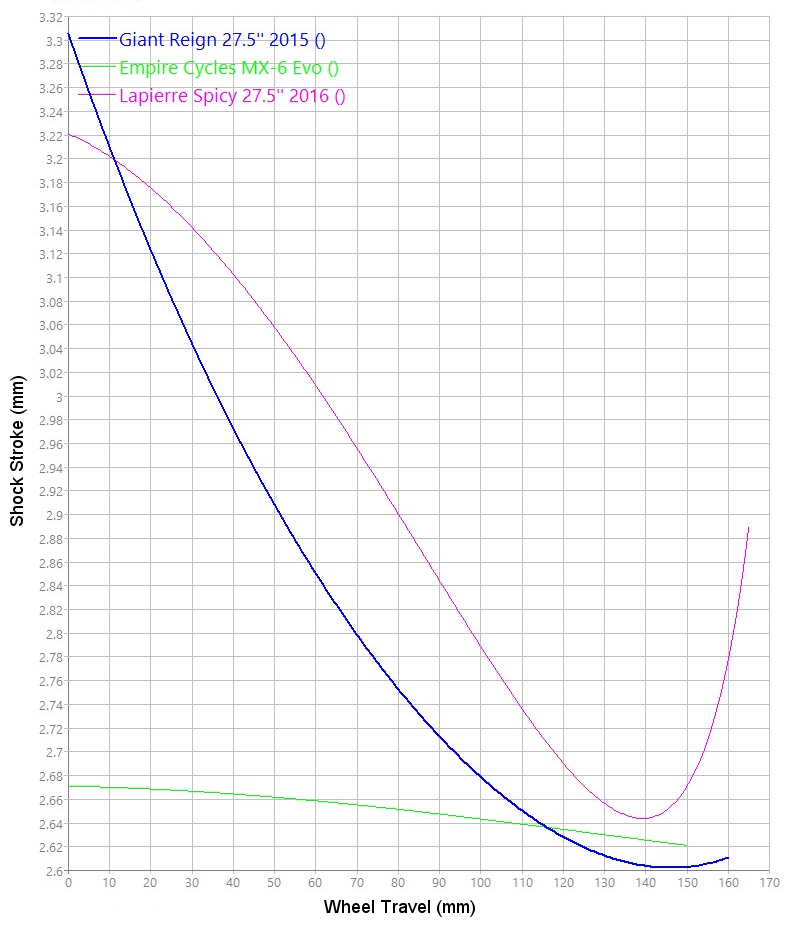
\includegraphics[width=10cm]{../images/3_bike_lev_ratio.jpg}
			\caption{Leverage curves of three modern suspension designs}
			\label{fig:3_bike_lev_ratio}
		\end{figure}
		\\
		The Virtual Pivot Point (VPP) design of the Giant Reign (shown blue) has an initial falling rate, meaning the shock can be compressed easily, but slows down and even rises slightly towards the end of its travel as seen in Figure \ref{fig:3_bike_lev_ratio}. This means the suspension will feel soft most of the time but stiffer as compression increases. This is emphasised by the Horst link system of the Lapierre Spicy (shown magenta) where the leverage curve rises significantly towards the end of its travel.In contrast, the curve of the single pivot Empire MX-6 Evo (shown green) is effectively linear. This is due to the MX-6 having only one pivot and swinging arm, as opposed to multiple pivots and linkages of the VPP and horst link designs, so there is an almost direct input from the rear wheel to the shock. The physical differences in each of these frames can be seen in Figure \ref{fig:3_bike_diagrams}.
		\begin{figure}[h!]
			\centering
			\begin{subfigure}[t]{0.3\textwidth}
				\centering
				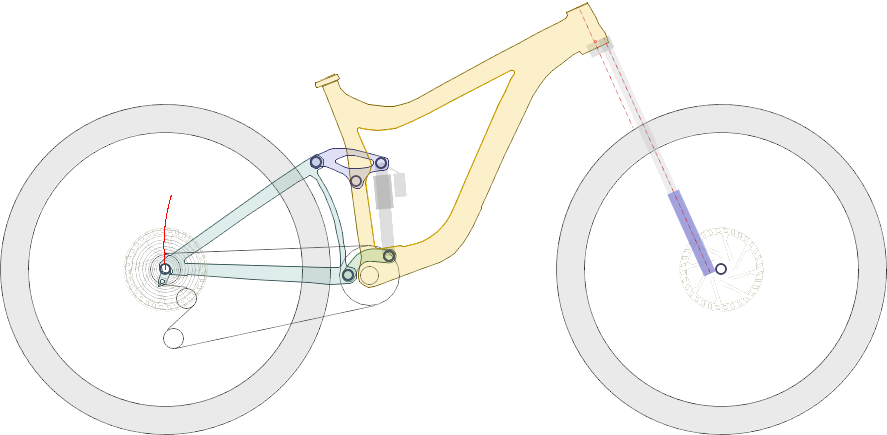
\includegraphics[width=\textwidth]{../images/3_bikes/giant.png}
				\subcaption{Giant Reign}
			\end{subfigure}
			\begin{subfigure}[t]{0.3\textwidth}
				\centering
				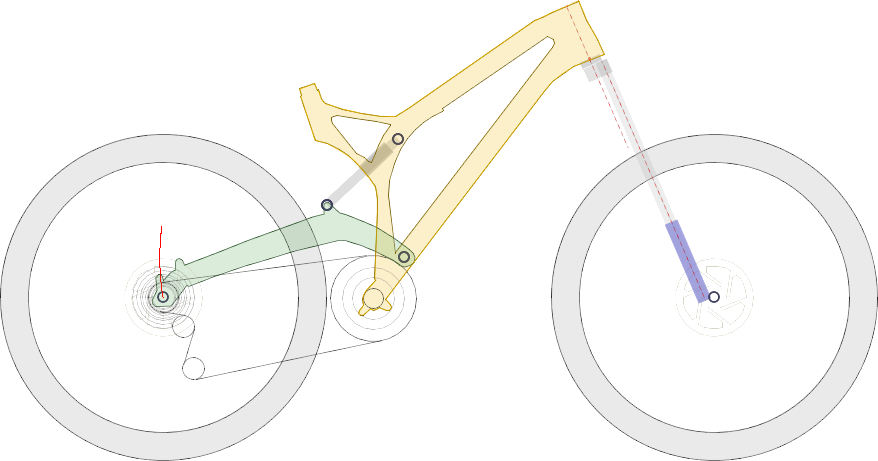
\includegraphics[width=\textwidth]{../images/3_bikes/empire.png}
				\subcaption{Empire MX6 Evo}
			\end{subfigure}
			\begin{subfigure}[t]{0.3\textwidth}
				\centering
				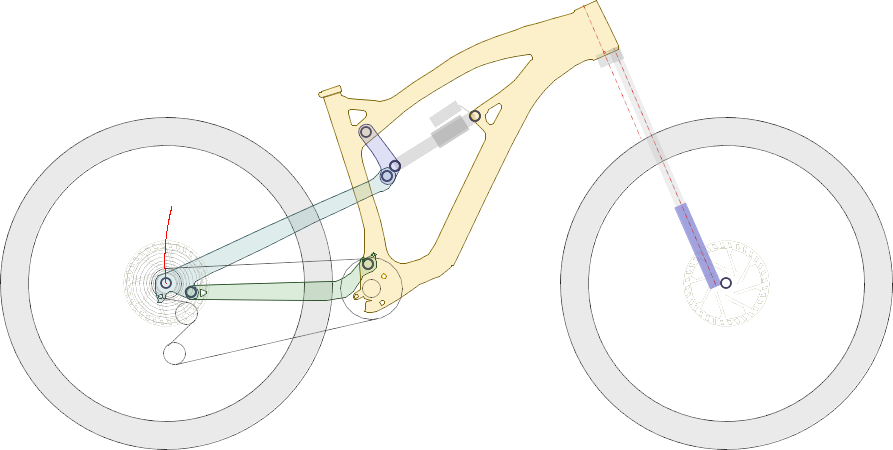
\includegraphics[width=\textwidth]{../images/3_bikes/lapierre.png}
				\subcaption{Lapierre Spicy}
			\end{subfigure}
			\caption{Full suspension frame comparison}
			\label{fig:3_bike_diagrams}
		\end{figure}
		\\
		For this project two bikes will be used for development and testing of the application. The first is a 2015 Giant Reign, shown on figure 3 in blue, as it will be constantly available throughout the project. The frame uses Giant’s Maestro™suspension system which is a variation of VPP. Like all VPP systems Maestro uses two links, an upper and lower, to create a virtual main pivot point, however unlike other VPP systems, Maestro creates its virtual pivot as close to the rear of the frame as possible As shown by the red circle in Figure \ref{fig:maestro}. The second will be a 2011 Orange 5 which has the same suspension design as the Empire MX6 Evo in Figure \ref{fig:3_bike_lev_ratio}. This bike was selected as it has a completely different design to the Giant Reign and will also be easily accessible throughout the project. 
		\begin{figure}[h!]
			\centering
			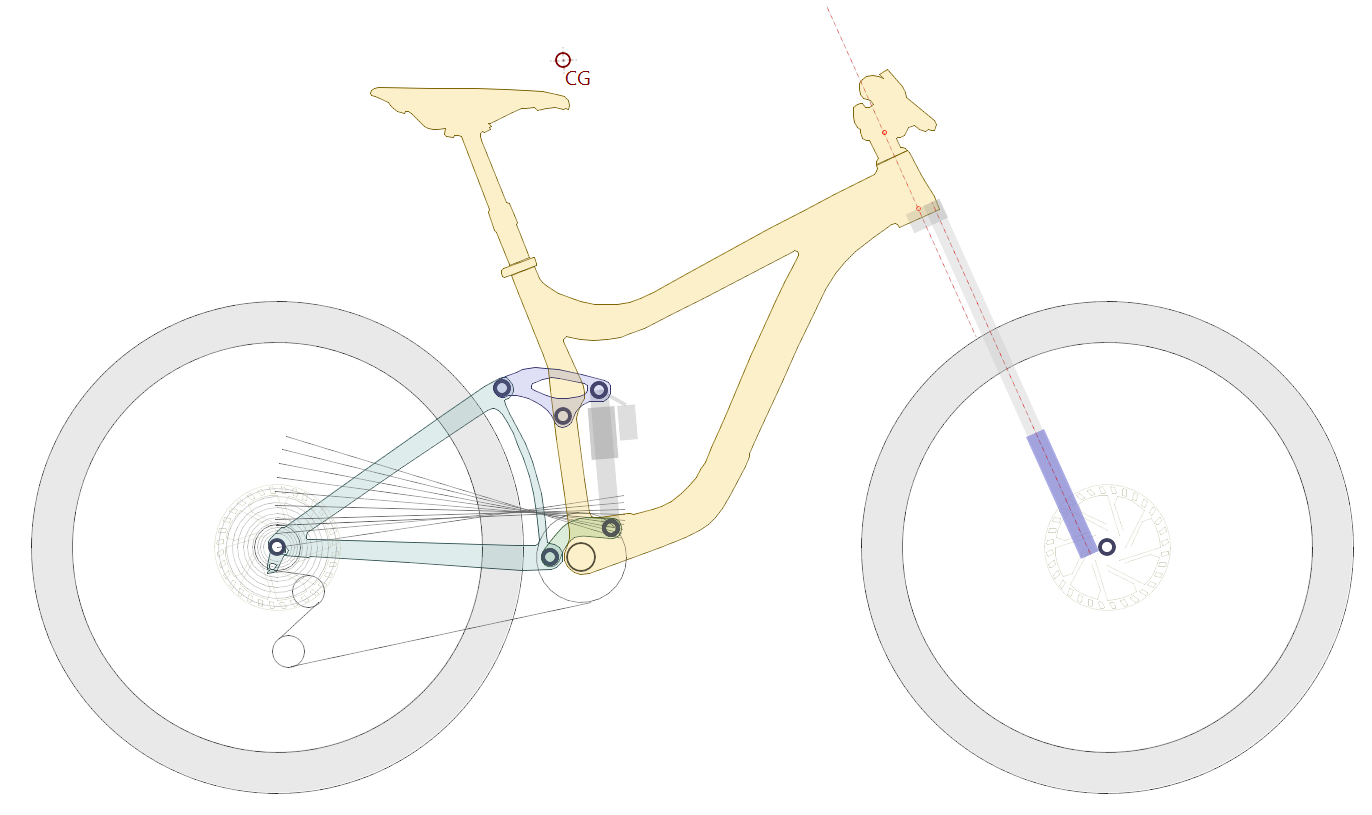
\includegraphics[width=12cm]{../images/reignsch.PNG}
			\caption{Maestro suspension}
			\label{fig:maestro}
		\end{figure}
		\\
		Although rear suspension designs are complex, neither the average rider nor professionals, such as mechanics, working in the industry necessarily need this specialist knowledge. Leverage curves are predominantly used by designers to determine how a particular suspension unit will behave when researching and designing new frames \citep{creek2016curves}. Though having an understanding of leverage curves will help the individual rider to fine tune their suspensions settings described in the following sections themselves, the majority will take little interest in the differences between a single pivot and VPP design, choosing a simpler ”set and forget” approach to their suspension. 
		\\\\
		In the context of this project and the intended user for the application, this begs the question of how much information should be provided to the user? Modern human /computer interaction principles aim toward providing information to the user which is relevant and necessary in context \citep{shneiderman2010designing}. Presenting the user with a leverage curve which may require extensive interpretation before they understand the implications within the limitations of a mobile application may prove detrimental to the user experience. For an application which is intended to remove the difficulties of suspension setup and allow for quick and easy production of a basic setup, providing a single sag setting would be preferable over a plethora of of technical data.	
	\subsubsection{Sag} \label{sec:sag}
		\todo{review section adding detail on setup method}
		Sag is the amount that the suspension sits into its travel when the rider is in a neutral position, described in Figure \ref{fig:sag}. It is required so that the suspension has travel available to extend as well as just compress and is calculated using the rider’s weight, available travel, and intended riding style.
		\\\\
		The amount of sag depends on the stiffness of the suspension unit which can be adjusted by changing the air pressure of an air spring or replacing the spring and adjusting the preload of a traditional coil shock. Depending on discipline and the	amount of travel the bike has, sag can vary between 15\% and 40\% of the available travel though it is typically set at between 25\% and 35\% for the average rider with greater variances only encountered in competition.
		\begin{figure}[h!]
			\centering
			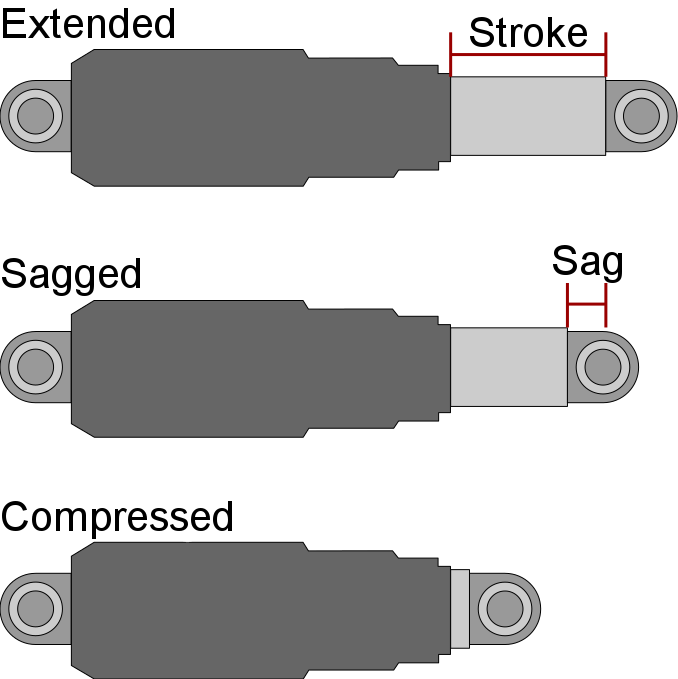
\includegraphics[scale=0.5]{../images/sag_diagram.png}
			\caption{Diagram of shock states indicating sag}
			\label{fig:sag}
		\end{figure}
		\\
		Sag is set by first calculating the distance that the shock should sit into its travel by producing the desired percentage of the shocks stroke. For an air shock the manufacturers recommended pressure is then pumped into the shock and the rider weights the bike. On each air shock there is a marker o-ring which is pushed down the shock shaft when the shock is compressed. The position this o-ring ends at can be measured and the shock pressure adjusted accordingly until it sits at the target measurement. 
	\subsubsection{Damping}
		In a spring and mass system, when the spring is elongated it will exert a returning force on the mass which, according to Hooke's law \citep{rychlewski1984hooke}, is directly proportionate to the distance which the spring has been pulled. In suspension this force is explained as two separate forces. If an individual were to push down on mountain bike suspension they would feel a resistance, this is known as compression, and when they let go the suspension will return to its neutral state, this is rebound. Both of these can be controlled which is known as damping.
		\\\\
		Suspension damping works by forcing oil within the shock absorber through a series of holes in the absorber’s damping circuit. Reducing the size or number	of holes increases resistance, reducing the speed at which the oil flows through the circuit to increase the damping effect by making compression and rebound slower.
	\paragraph{Compression Damping} 
		This is applied while the shock absorber is being compressed to control the effort required to do so. Increasing damping forces the wheel to remain in contact with the ground which makes the suspension feel stiffer. However too much compression damping can make the suspension overly stiff so it does not effectively absorb the impact of bumps and rough terrain. Conversely, too little compression damping can cause the suspension to ”blow through” all of the available travel prematurely with nothing left to soak up impact when it is most required. 
	\paragraph{Rebound Damping}
		This is used to control the speed at which the shock absorber recovers to its normal riding position after compression. An optimal setting will allow the suspension to track the ground, quickly and smoothly returning to the correct position after a bump or hole is passed. 
		\\\\
		Too much rebound damping causes the suspension unit to recover slowly and sometimes “pack down” meaning the shock absorber remains compressed for too long leaving the rider fully exposed to the next impact. Too little rebound damping can cause the suspension to “buck” the rider, like a horse, and potentially cause an accident.
	\paragraph{High and Low Speed Damping} 
		The ways of adjusting compression and rebound damping differ by manufacturer and model with better specified bikes having two adjustable speeds for each damping circuit giving four damping settings. High speed adjustments are used in high G-force situations such as riding large jumps or drops where compression needs to be set softer to absorb impacts and rebound set slower so the rider has time to recover without the equilibrium of the bike being upset.
		\\\\
		Low speed damping set ups are used against lower G-force movements such as rider weight shifts or long, slow compressions. Optimally compression is set stiffer as this type of feature can use a lot of travel and rebound damping set faster to deal with multiple features in quick succession.
	\subsubsection{Optimal Setup}
		Although setups will vary between rider, suspension system and discipline, there are some key principles that all riders should aim to achieve. Sag should be set to an appropriate measurement by adjusting the air pressure on air shocks or spring rating on coil shocks. Compression damping should feel soft and soak up bumps efficiently without excessive bottoming out. Rebound damping should be set to return as fast as possible without bucking the rider, which is normally somewhere in the middle of the two setting available with a slight bias towards the faster option.
		\\\\
		Attaining this optimal setup can be difficult for both beginners and intermediate riders as they lack experience and in-depth knowledge of suspension units and may not know how different frames react while being ridden. Knowing which measurements to make and the calculations required to correctly configure sag, compression and rebound settings are typically beyond the capabilities of this level of rider unless they have been previously trained by a professional or investigated the topic in detail for themselves.